%
% $Id: SANDExampleArticleNotstrict.tex,v 1.14 2004/08/18 23:53:35 rolf Exp $
%
% This is an example LaTeX file which uses the SANDreport class file.
% It shows how a SAND report should be formatted, what sections and
% elements it should contain, and how to use the SANDreport class.
% It uses the LaTeX article class, but not the strict option.
% It uses jpeg logos and files to show how pdflatex can be used
%
% Get the latest version of the class file and more at
%    http://www.cs.sandia.gov/~rolf/SANDreport
%
% This file and the SANDreport.cls file are based on information
% contained in "Guide to Preparing {SAND} Reports", Sand98-0730, edited
% by Tamara K. Locke, and the newer "Guide to Preparing SAND Reports and
% Other Communication Products", SAND2002-2068P.
% Please send corrections and suggestions for improvements to
% Rolf Riesen, Org. 9223, MS 1110, rolf@cs.sandia.gov
%
\documentclass[pdf,ps2pdf,12pt]{SANDreport}
\usepackage{amssymb}
\usepackage{amsmath}
\usepackage{parskip}
\usepackage{cancel}
\usepackage[FIGBOTCAP,normal,bf,tight]{subfigure}

% If you want to relax some of the SAND98-0730 requirements, use the "relax"
% option. It adds spaces and boldface in the table of contents, and does not
% force the page layout sizes.
% e.g. \documentclass[relax,12pt]{SANDreport}
%
% You can also use the "strict" option, which applies even more of the
% SAND98-0730 guidelines. It gets rid of section numbers which are often
% useful; e.g. \documentclass[strict]{SANDreport}



% ---------------------------------------------------------------------------- %
%
% Set the title, author, and date
%
\title{
Time Integration Algorithms for State-Based Peridynamics
}

\author{John, Dave and Mike?\\
Sandia National Laboratories \\
1515 Eubank SE \\
Albuquerque, NM 87185
}

    % There is a "Printed" date on the title page of a SAND report, so
    % the generic \date should generally be empty.
    \date{}


% ---------------------------------------------------------------------------- %
% Set some things we need for SAND reports. These are mandatory
%
\SANDnum{SAND2011-xxxx}
\SANDprintDate{October 2011}
\SANDauthor{John, Dave and Mike?\\ Multiscale Dynamic Materials Modelling \\}


% ---------------------------------------------------------------------------- %
% Include the markings required for your SAND report. The default is "Unlimited
% Release". You may have to edit the file included here, or create your own
% (see the examples provided).
%
% \include{MarkUR} % Not needed for unlimted release reports



% ---------------------------------------------------------------------------- %
% The following definition does not have a default value and will not
% print anything, if not defined
%
%\SANDsupersed{SAND1901-0001}{January 1901}


% ---------------------------------------------------------------------------- %
%
% Start the document
%
\begin{document}
    \maketitle

    % ------------------------------------------------------------------------ %
    % An Abstract is required for SAND reports
    %
    \begin{abstract}
    This report documents time integration algorithms (implicit and explicit) implemented for state-based peridynamics.  Implicit time integration documented here builds upon the state-based peridynamics model ~\cite{ref:pdStates.Silling} and linearization framework ~\cite{ref:pdLinearization.Silling} by Silling and relies upon knowledge of relevant material modulus states ~\cite{ref:statePlasticityMitchell} for computing entries in the Jacobian operator.    Results presented are in contrast with most application development work to date that has used explicit time integration and/or bond based peridynamics~\cite{ref:pdOriginal.Silling}.  The report informally introduces state based peridynamics, and presents a standard time integration strategy and Newton Raphson solution algorithm for a time step.  
    \end{abstract}


    % ------------------------------------------------------------------------ %
    % An Acknowledgement section is optional but important, if someone made
    % contributions or helped beyond the normal part of a work assignment.
    % Use \section* since we don't want it in the table of context
    %
    \clearpage
    \section*{Acknowledgement}

\noindent

    % ------------------------------------------------------------------------ %
    % The table of contents and list of figures and tables
    % Comment out \listoffigures and \listoftables if there are no
    % figures or tables. Make sure this starts on an odd numbered page
    %
    \clearpage
    \tableofcontents
    \listoffigures
    \listoftables

    % ---------------------------------------------------------------------- %
    % This is where the body of the report begins; usually with an Introduction
    %
    \SANDmain		% Start the main part of the report
\section{Introduction and Approach}\label{section:introduction}
    This report documents time integration algorithms (implicit and explicit) implemented for state-based peridynamics.  Implicit time integration documented here builds upon the state-based peridynamics model ~\cite{ref:pdStates.Silling} and linearization framework ~\cite{ref:pdLinearization.Silling} by Silling and relies upon knowledge of relevant material modulus states ~\cite{ref:statePlasticityMitchell} for computing entries in the Jacobian operator.    Results presented are in contrast with most application development work to date that has used explicit time integration and/or bond based peridynamics~\cite{ref:pdOriginal.Silling}.  The report informally introduces state based peridynamics, and presents a standard time integration strategy and Newton Raphson solution algorithm for a time step.   It is relatively self-contained provided the reader is familiar with state-based peridynamics.   A brief outline of the report follows.   



\section{Implicit Time Integration of Momentum Equation}
\subsection{Peridynamics Treatment of the Momentum Equation for Solids}
Solution algorithms used for the momentum equation under both finite element and peridynamic discretizations are very similar.   The internal force for peridynamics is identical to that used in nonlinear finite element codes in the sense that forces are summed at a point.  In quasi-statics, the balance of forces at a point  defines equilibrium, while in dynamics the sum of forces equals the product of density and acceleration at the point.  In each case, it is necessary to evaluate the sum of forces at a point arising from deformations of the solid.  The method for evaluation of this force at a point is what differentiates peridynamics~\cite{ref:pdOriginal.Silling, ref:pdStates.Silling} from local continuum mechanics. This section is a brief introduction to the the internal force vector associated with peridynamics with an emphasis on its relation to constitutive models.  

Using the state-based theory of peridynamics, the momentum equation is given as:
\begin{eqnarray}
\rho(x) \ddot{u}(x,t) &=& \int_{H(x)} \left\lbrace T(Y[x])\left\langle p-x \right\rangle  - T(Y[p]) \left\langle x-p \right\rangle \right\rbrace \,dV_p+ b(x,t) \nonumber \\ 
&=& f(Y[x],t)+b(x,t)\label{eq:pdMomentum}
\end{eqnarray}
The above equation is the peridynamics representation of Newton's 2nd law for the Lagrangian point $x$ and defines the internal force vector $f(Y[x],t)$.    The function $b(x,t)$ denotes a body force per unit volume.  $T(Y[x])$ is a vector force state function (to be defined later) and is somewhat analogous to the stress tensor in local continuum mechanics in the sense that it represents the material response due to deformations.  For a specific material $T(Y[x])$ would be represented by a constitutive model.  Note the notation $T(Y[x])$ is used to denote the force state dependency upon the deformation state $Y$ at the point $x$.  This dependency is used later to linearize the internal force vector about a deformation state $Y^0[x]$.  
\subsection{Newmark Algorithm}
Application of the Newmark scheme is well documented \cite{ref:functionalAnalysis.jnReddy, ref:femBook.bathe} but included here for completeness.
It consists of the following two estimates for the displacement $u(t)$ and its time derivative at time $t+\Delta t$.  
\begin{eqnarray}
\dot{u}^{n+1} &=& \dot{u}^{n} + \left[(1-\alpha)\ddot{u}^{n}+\alpha \ddot{u}^{n+1}\right] \Delta t \nonumber \\
u^{n+1} &=& {u}^{n} + \dot{u}^n \Delta t + \left[(\frac{1}{2}-\beta)\ddot{u}^{n}+\beta \ddot{u}^{n+1}\right](\Delta t)^2 \label{eq:newmarkApproximation}
\end{eqnarray}
Different levels of accuracy and stability are given through the careful selection of $\alpha$, $\beta$ and $\Delta t$.  Note that superscripts denote function values at  a particular step $n$ and point $x$ based upon the following definitions: 
\begin{eqnarray}
u^{n}     &=&u(x,t) \nonumber \\
u^{n+1} &=&u(x,t+\Delta t) \nonumber 
\end{eqnarray}
Similarly for the velocity and acceleration.  

The schematic shown in Figure~\ref{fig:incrementalConfiguration}(a) graphically illustrates the point $x$ and its displacement $u^n$.  When combined, $x$ and $u^n$ give the current location $y^n=x+u^n$  of point $x$ at step $n$.  

To complete the development, the momentum equation (Eq.~\ref{eq:pdMomentum}) is written for step $n+1$:
\begin{eqnarray}
\rho \ddot{u}^{n+1} = f^{n+1} + b^{n+1} \label{eq:momentumNP1}
\end{eqnarray}
where $ f^{n+1}=f(Y[x],t+\Delta t)$ and  $b^{n+1}=b(x,t+\Delta t)$.

Then $\ddot{u}^{n+1}$, obtained by solving Eq~\ref{eq:newmarkApproximation} (2nd equation),  is substituted into Eq~\ref{eq:momentumNP1}.  This leads to the following implicit equation for $u^{n+1}$:
\begin{eqnarray}
\rho {u}^{n+1} = \beta (\Delta t)^2 \left[f^{n+1} + b^{n+1}\right]+\rho \left[ {u}^{n} + \dot{u}^n \Delta t + (\frac{1}{2}-\beta)(\Delta t)^2 \ddot{u}^{n}\right] \label{eq:implicitMomentum}
\end{eqnarray}
While not explicitly indicated, both $f^{n+1}$ and $b^{n+1}$ depend upon ${y}^{n+1}$ and thus on ${u}^{n+1}$.  

\begin{figure}
\begin{center}
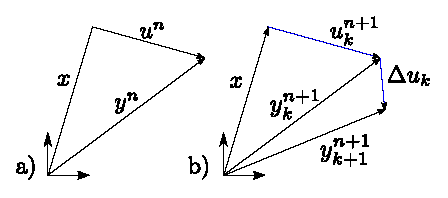
\includegraphics[scale=1.5]{figures/incrementalConfiguration.eps}
\end{center}
\caption{Incremental kinematics}
\label{fig:incrementalConfiguration}
\end{figure}

The above equation forms the basis of the incremental solution strategy.  The extent to which Eq~\ref{eq:implicitMomentum} is satisfied is measured by the associated residual equation:
\begin{eqnarray}
r({u}^{n+1}) = \rho {u}^{n+1}  - \beta (\Delta t)^2 \left[f^{n+1} + b^{n+1}\right]-\rho \left[ {u}^{n} + \dot{u}^n \Delta t + (\frac{1}{2}-\beta)(\Delta t)^2 \ddot{u}^{n}\right] \label{eq:implicitMomentumResidual}
\end{eqnarray}
The goal of the solution strategy for step $n+1$ is to find ${u}^{n+1}$ so that $\Vert r({u}^{n+1}) \Vert=0$.

\section{Incremental Solution Strategy for a Time Step}
Because the problem is in general non-linear, the incremental solution strategy for a load step consists of finding an increment, $\Delta u$, to the displacement ${u}^{n}$.  This is an iterative process; the following notation is used for iteration $k$ of a load step:
\begin{eqnarray}
{y}^{n+1}_{k+1}&=&x + {u}^{n+1}_{k} +\Delta u_k  \nonumber \\
                               &=&{y}^{n+1}_{k}+\Delta u_k\label{eq:incrementStrategy}            
\end{eqnarray}
where 
\begin{eqnarray}
{y}^{n+1}_{k}&=& x+{u}^{n+1}_{k}  \label{eq:incrementStrategy.ynp1.k}
\end{eqnarray}
In a typical Newton-Raphson strategy, ${u}^{n+1}_{k}$ is known from the previous iteration.  A graphical illustration of the kinematics for iteration $k$ is shown in Figure~\ref{fig:incrementalConfiguration}(b).   

To determine $\Delta u_k$, a Jacobian matrix associated with the internal force is required.  Using \eqref{eq:pdMomentum} and \eqref{eq:incrementStrategy.ynp1.k}, the internal force vector at step $n+1$ increment $k$ is defined as:
\begin{eqnarray}
{f}^{n+1}_{k}&=&f({Y}^{n+1}_{k},t+\Delta t)  \nonumber \\
                          &=& \int\left\lbrace T({Y}^{n+1}_{k}[x])\left\langle p-x \right\rangle  - T({Y}^{n+1}_{k}[p]) \left\langle x-p \right\rangle \right\rbrace \,dV_p\label{eq:pdIncrementalInternalForce}
\end{eqnarray}
Then, the first order approximation to $f^{n+1}_{k+1}$ is given as:
\begin{eqnarray}
{f}^{n+1}_{k+1}&\approx& {f}^{n+1}_{k}+Df(u^{n+1}_k)[\Delta u_k] \label{eq:directionalDerivativeI} \\     
                              &=& {f}^{n+1}_{k}+\int\left\lbrace (K[x]\bullet \Delta U_k[x])\left\langle p-x \right\rangle  - (K[p]\bullet \Delta U_k[p]) \left\langle x-p \right\rangle \right\rbrace \,dV_p \nonumber 
\end{eqnarray}
A special notation in \eqref{eq:directionalDerivativeI} is used to indicate the directional derivative of $f$ evaluated at $u^{n+1}_k$ in the direction $\Delta u_k$.  This is a linear operator with respect to $\Delta u_k$.
The second part of the above equation expresses the directional derivative of the internal force vector $f$ with respect to displacements $u$ in terms of an increment in the displacement state $ \Delta U$, where $K$ is the modulus state \cite{ref:pdStates.Silling} of the material evaluated at ${Y}^{n+1}_{k}$.  For implicit solution algorithms, evaluation of $K$ is crucial for optimal convergence rates.  The modulus state is a second order tensor that is material dependent.   For elastic, and elastic-plastic materials, analytical expressions are given for $K$~\cite{ref:statePlasticityMitchell}. 

\subsection{Newton Steps}
Given the residual Eq~\ref{eq:implicitMomentumResidual}, the linear problems associated with Newton iterations are defined as:
\begin{eqnarray}
0 & \approx & r({u}^{n+1}_{k+1}) \nonumber \\
   & \approx & r({u}^{n+1}_{k}) + \left . \frac{\partial r}{\partial {u}^{n+1}}\right\vert_{{u}^{n+1}_{k}} \cdot \Delta u_k \label{eq:newtonIteration}
\end{eqnarray}
Using Eq~\ref{eq:implicitMomentumResidual}, the directional derivative of the residual is:
\begin{eqnarray}
 \left . \frac{\partial r}{\partial {u}^{n+1}}\right\vert_{{u}^{n+1}_{k}} = \rho I -\beta ({\Delta t})^2 \left . \left( \frac{\partial f^{n+1}}{\partial {u}^{n+1}}+\frac{\partial b^{n+1}} {\partial {u}^{n+1}}\right)\right\vert _{{u}^{n+1}_{k}}
\end{eqnarray}
where $\left . \frac{\partial f}{\partial {u}^{n+1}}\right\vert_{{u}^{n+1}_{k}}$ is defined in Eq~\ref{eq:pdFirstOrderInternalForce}.  For completeness, the residual $r({u}^{n+1}_{k}) $ required for each Newton iteration is defined in Eq~\ref{eq:implicitMomentumResidual} and given by:
\begin{eqnarray}
r({u}^{n+1}_k) = \rho {u}^{n+1}_k  - \beta (\Delta t)^2 \left[f^{n+1}_k + b^{n+1}_k\right]-\rho \left[ {u}^{n} + \dot{u}^n \Delta t + (\frac{1}{2}-\beta)(\Delta t)^2 \ddot{u}^{n}\right] \label{eq:implicitMomentumResidualNewtonIterationK}
\end{eqnarray}
Note that values for the primary variable at step $n$ do not include a subscript since they are converged values from the last loadstep.

\section{Demonstration Calculations}

\section{Summary and Conclusions}

    % ---------------------------------------------------------------------- %
    % References
    %
%    \clearpage
    \bibliographystyle{plain}
    \bibliography{SAND2011-ImplicitReferences}
    \addcontentsline{toc}{section}{References}

%
% This is an example of how to create the distribution page. Some
% distributions are required by Sandia; e.g. the housekeeping copies.
% Depending on the type of report; e.g. CRADA, Patent Caution, etc.
% additional distribution lines may have to be added. See the
% "Guide for Preparing SAND Reports"
%
% SANDdistribution takes CA or NM as an optional argument. If given,
% the approrpiate housekeeping copies are inserted autmatically.
% Inside the SANDdistribution environment, several commands can be used
% insert the distributions for CRADA, LDRD, etc. See example below.
%
% You can leave the CA or NM option off and not use any of the SANDdist*
% commands. This will allow you to create a distribution list manually.
%
\begin{SANDdistribution}[NM]
    % Housekeeping copies necessary for every unclassified report:
    % \SANDdistCRADA	% If this report is about CRADA work
    % \SANDdistPatent	% If this report has a Patent Caution or Patent Interest
    % \SANDdistLDRD	% If this report is about LDRD work

    % The following MUST BE between the external and internal distributions!
    % \SANDdistClassified % If this report is classified

    % Internal Addresses
    \SANDdistInternal{1}{1322}{John Aidun}{1425}
    \SANDdistInternal{1}{1320}{Scott Collis}{1442}
    \SANDdistInternal{1}{0372}{Eliot Fang}{1524}
    \SANDdistInternal{1}{0372}{Mike Glass}{1545}
    \SANDdistInternal{1}{1318}{Bruce Hendrickson}{1440}    
    \SANDdistInternal{1}{1318}{Robert Hoekstra}{1426}    
    \SANDdistInternal{1}{0380}{Joe Jung}{1542}
    \SANDdistInternal{1}{0825}{Joel Lash}{1510}
    \SANDdistInternal{1}{1322}{David Littlewood}{1444}
    \SANDdistInternal{1}{1322}{John Mitchell}{1444}
    \SANDdistInternal{1}{1322}{Rick Muller}{1425}    
    \SANDdistInternal{1}{0316}{Larry Musson}{1425}
    \SANDdistInternal{1}{1320}{Michael Parks}{1444}
    \SANDdistInternal{1}{1318}{Roger Pawlowski}{1444}
    \SANDdistInternal{1}{1318}{Eric Phipps}{1441}    
    \SANDdistInternal{1}{9042}{Jake Ostien}{8246}
    \SANDdistInternal{1}{1318}{Andy Salinger}{1442}
    \SANDdistInternal{1}{1321}{Randall Summers}{1444}
    \SANDdistInternal{1}{0380}{David Womble}{1540}

    % Example of a mail channel use (instead of a mail stop)
%    \SANDdistInternalM{1}{M9999}{Someone}{01234}

\end{SANDdistribution}

\begin{SANDdistribution}
\SANDdistInternal{1}{0899}{Technical Library}{9536}
\end{SANDdistribution}
\end{document}
